\section{Introduction}
%	\textcolor{red}{Change this section} \\
%	A qubit is the most elementary unit in quantum information. It is the quantum equivalent of the bit in classic computing and  can be described simply as a two-level quantum system. While a classic bit can take only one of two values described as 0 and 1, a qubit can exist in a superposition of these values, which allows it theoretically to have an infinite number of states.\\
%	There are multiple physical manifestations for qubits implemented in quantum systems today, such as charge in Josephson junction or the direction of the spin of an electron or the polarization state of a photon, and so on. Here in this work, we explore the usage of photonic qubits. The advantage of photonic qubits is the ability to manipulate them at room temperature and less prone to interact with their environment. To obtain photonic qubits, we need to have a single photon source which is one of the fundamental requirements in  quantum optical technologies.\\
%	One of the best candidates for such a source is self-assembled quantum dots (QDs). A QD can provide an optically controlled source of on-demand single photon source with well-defined polarization. We can use multiple methods in QD to define a two-level system; here, we choose the exciton and biexciton and study them by measuring the correlation between them.  
	
  	\subsection{Self assembled QDs}
	Self-assembled quantum dots (QDs) are localized nano-scale semiconductor structures that creates a three-dimensional(3D) potential well, both in the valence and conduction bands,which trap charge carriers. Due to their small confinement length relative to the particle's wavelength, the energy levels of the QD are quantized with properties similar to atoms which lead them to be described as "Artificial Atoms" \cite{Kastner1993}. \\
In recent years, semiconductor QDs were thoroughly investigated as technology-compatible single photon sources, providing a quantum source of "flying qubits" on demand.\cite{Dekel2000,Michler2000,Michler2000_1,Yuan2002} Moreover, recently it has been shown that QDs can emit pair of entangled photons \cite{Akopian2006,Hafenbrak2007} and that an emitted photon can be entangled with the remaining spin in the QD. \cite{Pelk2012,Schaibley2013,Gao2012} These achievements form the required building blocks for quantum information processing. \cite{DiVincenzo1998,Duan2001}\\
In semiconductor QDs, at low temperatures, the basic optical excitation, in which an electron is optically excited from the full valence band, thereby leaving there a hole, to the empty conduction band is called a bright exciton(BE). In self-assembled QDs the BE consists of an electron - heavy-hole pair.This optical excitation preserve the spin orientation of the excited electron and therefore the electron and hole are said to have anti-parallel spins. The total angular momentum projection of the BE on the direction of the exciting light is therefore ±1 (like that of the absorbed photon), reflecting the orbital momentum difference between the electron in the valence band to that in the conduction band.
If the excited conduction electron's spin projection is in addition opposite to the spin projection of the ground valence band electron the electron and the 2 hole have parallel spins, with total angular momentum projection of ±2. This type of excitation is optically forbidden since the light electric field cannot change the electronic spin and therefore it is called dark exciton (DE).Excitons in the QD can be generated also while the QD contains additional charges, such as a single electron or a single hole. Similarly, many other types of multiple carrier configurations can populate the QD at a given time. For example, a biexciton is two excitons (two electrons and two holes), and a positively (negatively) charged exciton (trion) is an exciton with addition of one hole (electron), just to mention a few basic QD excitations.

\subsection{The QD exciton fine structure}
Figure \ref{fig:energy_structure}  presents the four lowest energy configurations of electron-heavy hole pairs (excitons) and describes the energy difference between the parallel and anti-parallel spin configurations. The energy splitting between the DE and the BE is $\triangle_0 \approx 300 \mu eV$ due to the isotropic long and short range electron-hole exchange interaction (EHEI). Additional splitting is caused by the anisotropic (mainly long range) EHEI which removes the degeneracy between the two BE eigenstates by $\triangle_2 \approxeq 30 \mu eV $.The BE eigenstates are the symmetric and the antisymmetric configurations of the electron and hole with anti-parallel spins $ \ket{S}_{BE} = (\ket{\uparrow\Downarrow}+(\downarrow\Uparrow))/\sqrt{2}$ and  $ \ket{A}_{BE} = (\ket{\uparrow\Downarrow}-(\downarrow\Uparrow))/\sqrt{2}$ respectively. Here, a single arrow represents an electron and a double-arrow represents a heavy-hole in their respective ground levels. The DE eigenstates, similar to that of the BE, are the symmetric and the anti-symmetric configurations of the electron–hole pair with parallel spins $ \ket{S}_{DE} = (\ket{\uparrow\Uparrow}+(\downarrow\Downarrow))/\sqrt{2}$ and $ \ket{A}_{DE} = (\ket{\uparrow\Uparrow}-(\downarrow\Downarrow))/\sqrt{2}$.
\begin{figure}[H]
	\centering
	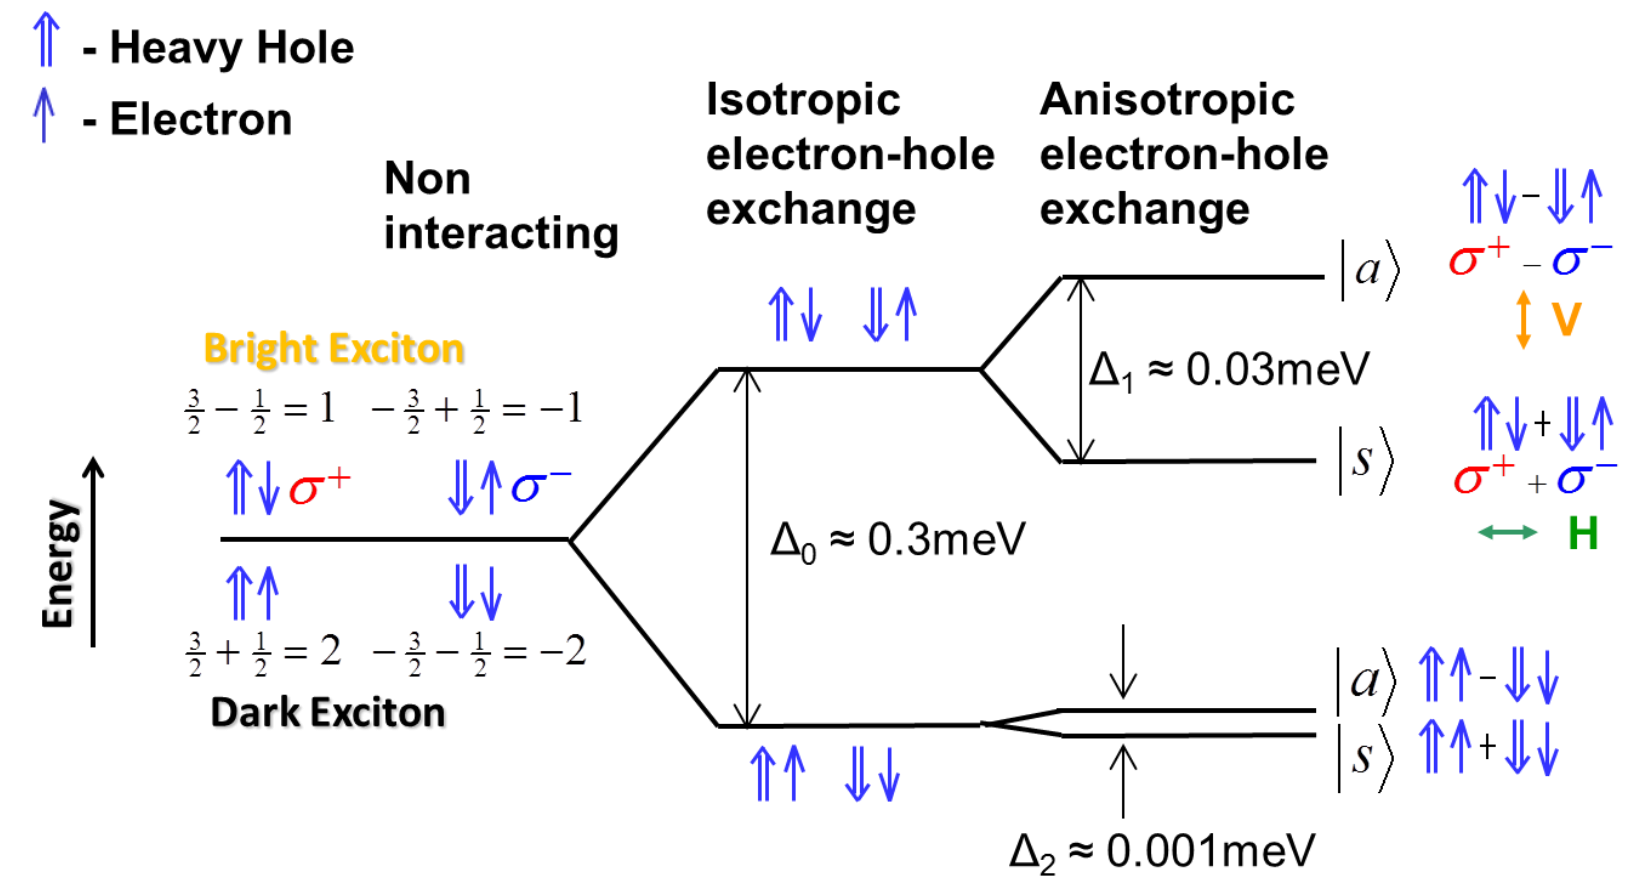
\includegraphics[scale=0.32]{figures/energy_structure.png}
	\caption{Schematic description of the bright and dark exciton energy levels and spin eigenstates. The polarization of light that interacts with the BE eigenstates is marked underneath the corresponding BE eigenstate.}
	\label{fig:energy_structure}
\end{figure}
Both the BE and DE thus have two non-degenerate spin eigenstates and both can, under some approximation, be considered as an isolated physical two level system. An exciton in an eigenstate will eventually decay. The BE which isoptically allowed, decays radiatively within $\approx$1 ns.


	The projection of the spin of the electron on the z-axis (growth axis) of the QD can be either 1/2 or -1/2 while for the heavy hole, the spin 
 projection is either 3/2 or -3/2 such that the two spin states of the bright exciton are $\ket{\frac{1}{2},-\frac{2}{3}}$ and $\ket{-\frac{1}
 {2},\frac{2}{3}}$  with a total spin in the z direction  of $\pm1$. While in the case of electron-hole pair with parallel spin, the spin states are $\ket{\frac{1}{2},\frac{2}{3}}$ and $\ket{-\frac{1}{2},-\frac{2}{3}}$ with a total spin of $\pm2$.\\
	In figure \ref{fig:energy_levels} we describe two of the simple configurations that we can have in a QD. We start with empty dot which we denote by $\ket{0}$.
	\begin{figure}[H]
		\centering
		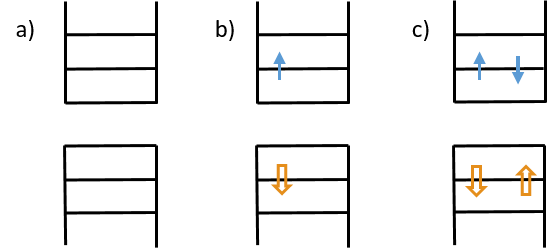
\includegraphics[scale=1]{figures/energy-levels.png}
		\caption{Schematic of the energy levels in the quantum dot for empty quantum dot (a),exciton (b) and a biexciton (c)}
		\label{fig:energy_levels}
	\end{figure}
	while having two electron-hole pairs falling in the dot a biexciton is formed and we denote it by $\ket{{XX}_0}$. The total energy of the biexciton differs from twice the energy of the exciton due to the interaction between all the particles.\\
	
	In an ideal QD, the radiative decay path of the biexciton back to the ground state goes via one path, but due to the anisotropy of the QD, the energy of exciton is split in what is defined as the fine structure splitting (FSS) as seen in figure \ref{fig:figureDecay_paths}b. Here we refer to the up (down) spin of the electron as $\ket{\uparrow}$ ($\ket{\downarrow}$ and the up (down) spin of the hole as $\ket{\Uparrow}$ ($\ket{\Downarrow}$ such as the two eigenstates of the exciton are  $\ket{\uparrow\Downarrow}$ and $\ket{\downarrow\Uparrow}$,and the decay from these states result in the emission of photons with co-linear polarization. Here we refer to them as horizontal $\ket{H}$ and vertical $\ket{V}$. We can represent these two rectilinear bases using the Bloch sphere where the poles in the sphere are $\ket{H}$ and $\ket{V}$ base.\\
	
	In addition to the rectilinear polarization states, We can define the diagonal linear and
	the circular polarization bases: 
	\begin{equation}
		\begin{split}
			\ket{L}=(\ket{H}+i\ket{V})/\sqrt{2} \\
			\ket{R}=(\ket{H}-i\ket{V})/\sqrt{2}
		\end{split}
	\end{equation}
	where $\ket{R}$ and $\ket{L}$ are the left and right circular bases respectively, and:
	\begin{equation}
		\begin{split}
			\ket{D}=(\ket{H}+\ket{V})/\sqrt{2}\\
			\ket{\bar{D}}=(\ket{H}+\ket{V})/\sqrt{2}
		\end{split}
	\end{equation}
	$\ket{D}$ and $\ket{\bar{D}}$ are the diagonal and anti-diagonal bases respectively
	
	\begin{figure}[H]
		a)
		\raggedleft
		\def\psiLat{0}
		\def\psiLon{-50}
		\begin{blochsphere}[radius=2.5 cm,tilt=20,rotation=-20,opacity=0]
			\labelLatLon{psi}{\psiLat}{-\psiLon};
			\draw[-latex] (0,0) -- (psi) node[above]{$\large\ket{\psi}$};
			\drawRotationLeft[scale=0.9,style={red}]{0}{0}{0}{15}
			
			\drawGreatCircle[style={dashed}]{0}{0}{0}
			\drawBallGrid[style={opacity=0.5}]{30}{30}
			\draw [fill] (0,0) circle (1.5pt);
			\drawGreatCircle[style={dashed}]{0}{0}{0}
			\labelLatLon{up}{90}{0};
			\labelLatLon{down}{-90}{90};
			\node[above] at (up) {{ $\ket{H}$ }};
			\node[below] at (down) {{ $\ket{V}$}};
			\node at (2.8,0) {{$\ket{R}$}};
			\node at (-2.8,0) {{$\ket{L}$}};
			\node at (0,1) {{$\ket{D}$}};
			\node at (0,-1) {{$\ket{\bar{D}}$}};
		\end{blochsphere}
		b)
		\raggedright
		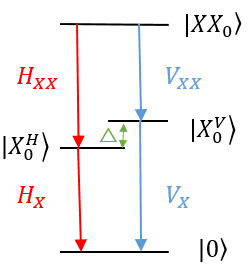
\includegraphics[scale=0.8]{figures/Decay_paths.png}
		\caption{a) A Bloch sphere representation of the spin state. A point on the sphere represents an arbitrarily polarized spin state. b) Decay paths of the biexciton back the ground state where the red arrows represent the emission of a H polarized photon and blue arrows represent the emission of V polarized photon.}
		\label{fig:Decay_paths}
	\end{figure}
	When the biexciton spontaneously radiatively decays it  emits a photon leaving 
	in the QD an exciton in coherent superposition of its two eigenstates. The optical
	selection rules for the biexciton radiative recombination and the lack of information by “which path” the recombination proceeds result in entanglement between the exciton state and the polarization state of the emitted photon. Their mutual wave function is given by:
	\begin{equation}
		\ket{\psi_{X^0}} = \frac{1}{\sqrt{2}}(\ket{H_1H^1_H} +\ket{V_1V^1_V})
	\end{equation}
	here $\ket{H_1}$ and $\ket{V1}$ are the two rectilinear polarization states of the first (biexciton) photon. since the two exciton eigenstates are not degenerate, the relative phase between these eigenstates precesses in time with a period of $T_P = h/\triangle$, where where $h$ is the Planck constant and $\triangle$ is the exciton FSS \cite{rwinik2017}.
	This precession is schematically described on the exciton Bloch sphere in figure. $\ref{fig:Decay_paths}a$.
	The precession “stops” when the exciton recombines and the radiative cascade is completed with the emission of a second photon. The two photons are thus entangled. Their mutual wave function depends on the recombination time and is given by:
	\begin{equation}
		\ket{\psi_{X^0}} = \frac{1}{\sqrt{2}}(\ket{H_1H_1} +e^{-i2\pi t/T_P}\ket{V_1V_2})
	\end{equation}
 
	where $\ket{H_2}$ and $\ket{V_2}$ are the second (exciton) photon polarization states and $t = t_{X_0} - t_{{XX}_0}$ is the time between the emission of the biexciton photon $t_{{XX}_0}$ and that of the exciton $t_{X_0}$.